\documentclass[12pt,ngerman,parskip=half]{scrartcl}

\usepackage[utf8]{inputenc}
\usepackage[T1]{fontenc}
\usepackage{babel}
\usepackage{tikz}

\usepackage[]{pgfplots}
\pgfplotsset{width=15cm,compat=1.18}
\begin{document}

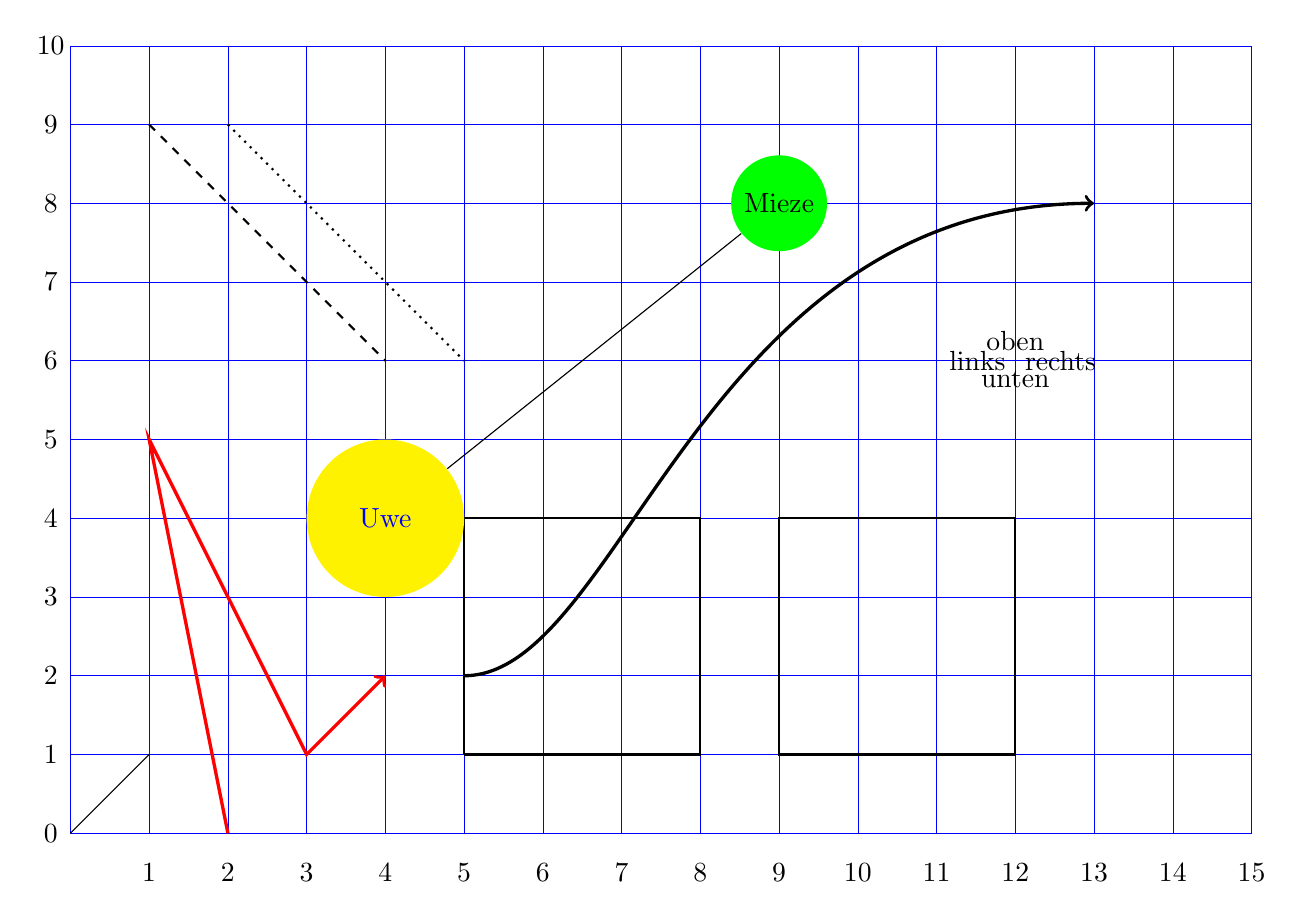
\begin{tikzpicture}[
punkt/.style={circle, minimum size = 2cm, blue, fill=yellow},
kleinpunkt/.style={punkt, minimum size = 1cm, black, fill=green},
]

\draw[help lines,blue,step=1cm] (0,0) grid (15,10);
\foreach \xtick in {1,...,15} {\pgfmathsetmacro\result{\xtick} \node at (\xtick,-0.5) {\pgfmathprintnumber{\result}}; }
\foreach \ytick in {0,...,10} {\pgfmathsetmacro\result{\ytick} \node at (-0.25,\ytick) {\pgfmathprintnumber{\result}}; }

\draw (0,0) -- (1,1);

%mit absoluten und relativen Koordinaten
\draw[->,very thick,red] (2,0) -- (1,5) -- (3,1) -- ++(1,1);

\draw[black, thick] (5,1) -- (5,4) -- (8,4) -- (8,1) -- (5,1); 

\draw[black, thick] (9,1) --  ++(0,3) -- ++(3,0) -- ++(0,-3) -- cycle; 

\draw[->,black,very thick] (5,2) .. controls (7,2) and (8,8) .. (13,8);

\node[punkt] (A) at (4,4){Uwe};
\node[kleinpunkt] (B) at (9,8){Mieze};

\draw (A) -- (B);

\draw[thick,black,dashed] (1,9) -- ++ (3,-3);

\draw[thick,black,dotted] (2,9) -- ++ (3,-3);

\node [below] at (12,6) {unten};
\node [above] at (12,6) {oben};
\node [left] at (12,6) {links};
\node [right] at (12,6) {rechts};

\end{tikzpicture}


% Preamble: \pgfplotsset{width=7cm,compat=1.18}
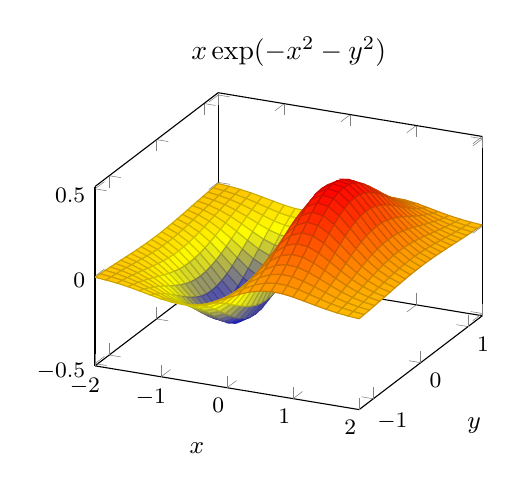
\begin{tikzpicture}
\begin{axis}[
title={$x \exp(-x^2-y^2)$},
xlabel=$x$, ylabel=$y$,
small,
]
\addplot3 [
surf,
domain=-2:2,
domain y=-1.3:1.3,
] {exp(-x^2-y^2)*x};
\end{axis}
\end{tikzpicture}


\end{document}

[
punkt/.style={circle, minimum size = 2cm, blue, fill=yellow},
kleinpunkt/.style={punkt, minimum size = 1cm, black, fill=green},
]
\draw[help lines,blue] (0,0) grid (15,10);

\draw (0,0) -- (1,1);

\draw[->,very thick] (2,0) -- (1,5);

\draw[->] (6,1) .. controls (7,2) and (8,8) .. (9,3);

\node[punkt] (A) at (4,4){U};
\node[kleinpunkt] (B) at (10,9){Z};

\draw (A) -- (B);
